	
\begin{minipage}[t]{7 cm}
		\emph{Dans cet exercice, aucune justification n'est demandée.}
		
		On a construit un carré ABCD. 
		
		\smallskip
		
		On a construit le point O sur la droite (DB), à
		l'extérieur du segment [DB] et tel que : OB = AB.
		
		\smallskip
		
		Le point H est le symétrique de D par rapport à O.
		
		\bigskip
		
		On a obtenu la figure ci-contre en utilisant plusieurs
		fois la même rotation de centre O et d'angle 45°.
		
		\bigskip
		
		La figure obtenue est symétrique par rapport à l’axe
		(DB) et par rapport au point O.
\end{minipage}
	\hfill
	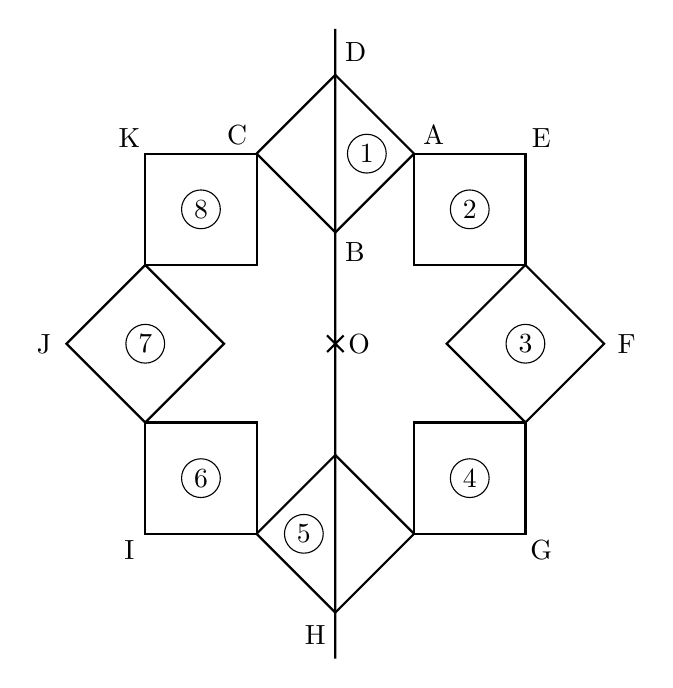
\begin{tikzpicture}[baseline={(D)}]
		\foreach \a in {0,45,...,315}
			\draw [line width=0.8pt] (0+\a:1.414)--++(-45+\a:1.414)--++(45+\a:1.414)--++(135+\a:1.414)--cycle;
		\foreach \a/\l in {2/E,3/F,4/G,6/I,7/J,8/K}
			\draw (135-\a*45:2.414) circle (7pt) node {\a}
			(135-\a*45:3.7) node{\l};
		\draw (0.4,2.414) circle (7pt) node {1};
		\draw (-0.4,-2.414) circle (7pt) node {5};
		\draw[line width=0.8pt] (0,-4)--(0,4) 
		(-3pt,-3pt)--(3pt,3pt) (-3pt,3pt)--(3pt,-3pt) (1pt,0)node[right] {O};
		\node (A) at (67.5:2.6) [above right]{A};
		\node (B) at (90:1.414) [below right] {B};
		\node (C) at (112.5:2.6) [above left] {C};
		\node (D) at (90:3.7) [right] {D};
		\node (H) at (-90:3.7) [left] {H};
	\end{tikzpicture}

	\begin{enumerate}
		\item Donner deux carrés différents, images l’un de l’autre par la symétrie axiale d’axe (DB).
		
		\item Le carré \tikz[baseline=(x.base)]{\draw (0,0) circle (7pt) node (x) {3};} est-il l’image du carré \tikz[baseline=(x.base)]{\draw (0,0) circle (7pt) node (x) {8};} par la symétrie centrale de centre O ?
		
		\item On considère la rotation de centre O qui transforme le carré \tikz[baseline=(x.base)]{\draw (0,0) circle (7pt) node (x) {1};} en le carré \tikz[baseline=(x.base)]{\draw (0,0) circle (7pt) node (x) {2};}.
		
		Quelle est l’image du carré \tikz[baseline=(x.base)]{\draw (0,0) circle (7pt) node (x) {8};} par cette rotation ?
		
		\item On considère la rotation de centre O qui transforme le carré \tikz[baseline=(x.base)]{\draw (0,0) circle (7pt) node (x) {2};} en le carré \tikz[baseline=(x.base)]{\draw (0,0) circle (7pt) node (x) {5};}.
		
		Préciser l’image du segment [EF] par cette rotation.
	\end{enumerate}

\bigskip

